\documentclass[handout]{beamer}\usepackage[]{graphicx}\usepackage[]{color}
%% maxwidth is the original width if it is less than linewidth
%% otherwise use linewidth (to make sure the graphics do not exceed the margin)
\makeatletter
\def\maxwidth{ %
  \ifdim\Gin@nat@width>\linewidth
    \linewidth
  \else
    \Gin@nat@width
  \fi
}
\makeatother

\definecolor{fgcolor}{rgb}{0.345, 0.345, 0.345}
\newcommand{\hlnum}[1]{\textcolor[rgb]{0.686,0.059,0.569}{#1}}%
\newcommand{\hlstr}[1]{\textcolor[rgb]{0.192,0.494,0.8}{#1}}%
\newcommand{\hlcom}[1]{\textcolor[rgb]{0.678,0.584,0.686}{\textit{#1}}}%
\newcommand{\hlopt}[1]{\textcolor[rgb]{0,0,0}{#1}}%
\newcommand{\hlstd}[1]{\textcolor[rgb]{0.345,0.345,0.345}{#1}}%
\newcommand{\hlkwa}[1]{\textcolor[rgb]{0.161,0.373,0.58}{\textbf{#1}}}%
\newcommand{\hlkwb}[1]{\textcolor[rgb]{0.69,0.353,0.396}{#1}}%
\newcommand{\hlkwc}[1]{\textcolor[rgb]{0.333,0.667,0.333}{#1}}%
\newcommand{\hlkwd}[1]{\textcolor[rgb]{0.737,0.353,0.396}{\textbf{#1}}}%

\usepackage{framed}
\makeatletter
\newenvironment{kframe}{%
 \def\at@end@of@kframe{}%
 \ifinner\ifhmode%
  \def\at@end@of@kframe{\end{minipage}}%
  \begin{minipage}{\columnwidth}%
 \fi\fi%
 \def\FrameCommand##1{\hskip\@totalleftmargin \hskip-\fboxsep
 \colorbox{shadecolor}{##1}\hskip-\fboxsep
     % There is no \\@totalrightmargin, so:
     \hskip-\linewidth \hskip-\@totalleftmargin \hskip\columnwidth}%
 \MakeFramed {\advance\hsize-\width
   \@totalleftmargin\z@ \linewidth\hsize
   \@setminipage}}%
 {\par\unskip\endMakeFramed%
 \at@end@of@kframe}
\makeatother

\definecolor{shadecolor}{rgb}{.97, .97, .97}
\definecolor{messagecolor}{rgb}{0, 0, 0}
\definecolor{warningcolor}{rgb}{1, 0, 1}
\definecolor{errorcolor}{rgb}{1, 0, 0}
\newenvironment{knitrout}{}{} % an empty environment to be redefined in TeX

\usepackage{alltt}

\usecolortheme[RGB={0,0,144}]{structure}
\usetheme{AnnArbor}\usecolortheme{beaver}

\usepackage{verbatim,xmpmulti,color,multicol,multirow}
\setlength{\unitlength}{\textwidth}  % measure in textwidths
\usepackage[normalem]{ulem}

\graphicspath{{../../include/}{../figs/}{../KState/}}

%\usepackage{beamerthemesplit}
\setbeamertemplate{navigation symbols}{}
\setbeamertemplate{enumerate items}[default]
\setbeamertemplate{enumerate subitem}{\alph{enumii}.}
\setbeamertemplate{enumerate subsubitem}{\roman{enumiii}.}
\setkeys{Gin}{width=0.6\textwidth}


\providecommand{\e}{\varepsilon}
\providecommand{\nv}{{}^{-1}}
\providecommand{\ov}[1]{\overline{#1}}
\providecommand{\q}{$\quad$ \newline}
\providecommand{\rt}{\rightarrow}
\providecommand{\vc}[1]{\boldsymbol{#1}}
\providecommand{\wh}[1]{\widehat{#1}}


\title[Bayesian RNAseq heterosis ]{Bayesian analysis for heterosis detection in RNAseq data}
\author[Jarad Niemi]{Dr. Jarad Niemi \\ joint with Eric Mittman, Will Landau, and Dr. Dan Nettleton}
\institute[Iowa State]{Iowa State University}
\date{\today}
\IfFileExists{upquote.sty}{\usepackage{upquote}}{}
\begin{document}

%\section{Temp??} \begin{comment}



\frame{\titlepage  
{\tiny
This research was supported by National Institute of General Medical Sciences (NIGMS) of the National Institutes of Health and the joint National Science Foundation / NIGMS Mathematical Biology Program under award number R01GM109458. The content is solely the responsibility of the authors and does not necessarily represent the official views of the National Institutes of Health or the National Science Foundation.
}}

\begin{frame}
\frametitle{Outline}

\begin{itemize}
\item Data
  \begin{itemize}
  \item Phenotypic heterosis
  \item RNAseq
  \end{itemize}
\item Methodology
  \begin{itemize}
  \item Model
  \item Empirical Bayes
  \item Stan
  \end{itemize}
\item Results
  \begin{itemize}
  \item Simulation study vs {\tt edgeR}, {\tt baySeq}, Ji et. al., {\tt ShrinkBayes}
  \item Real data analysis
  \end{itemize}
\item Fully Bayesian analysis
  \begin{itemize}
  \item GPUs
  \item Minimizing data transfer
  \item Slice sampling
  \end{itemize}
\end{itemize}

\end{frame}



\section{Data}
\subsection{Phenotypic heterosis}

\begin{frame}
\frametitle{Phenotypic heterosis in maize}
\setkeys{Gin}{width=0.8\textwidth}
\begin{center}
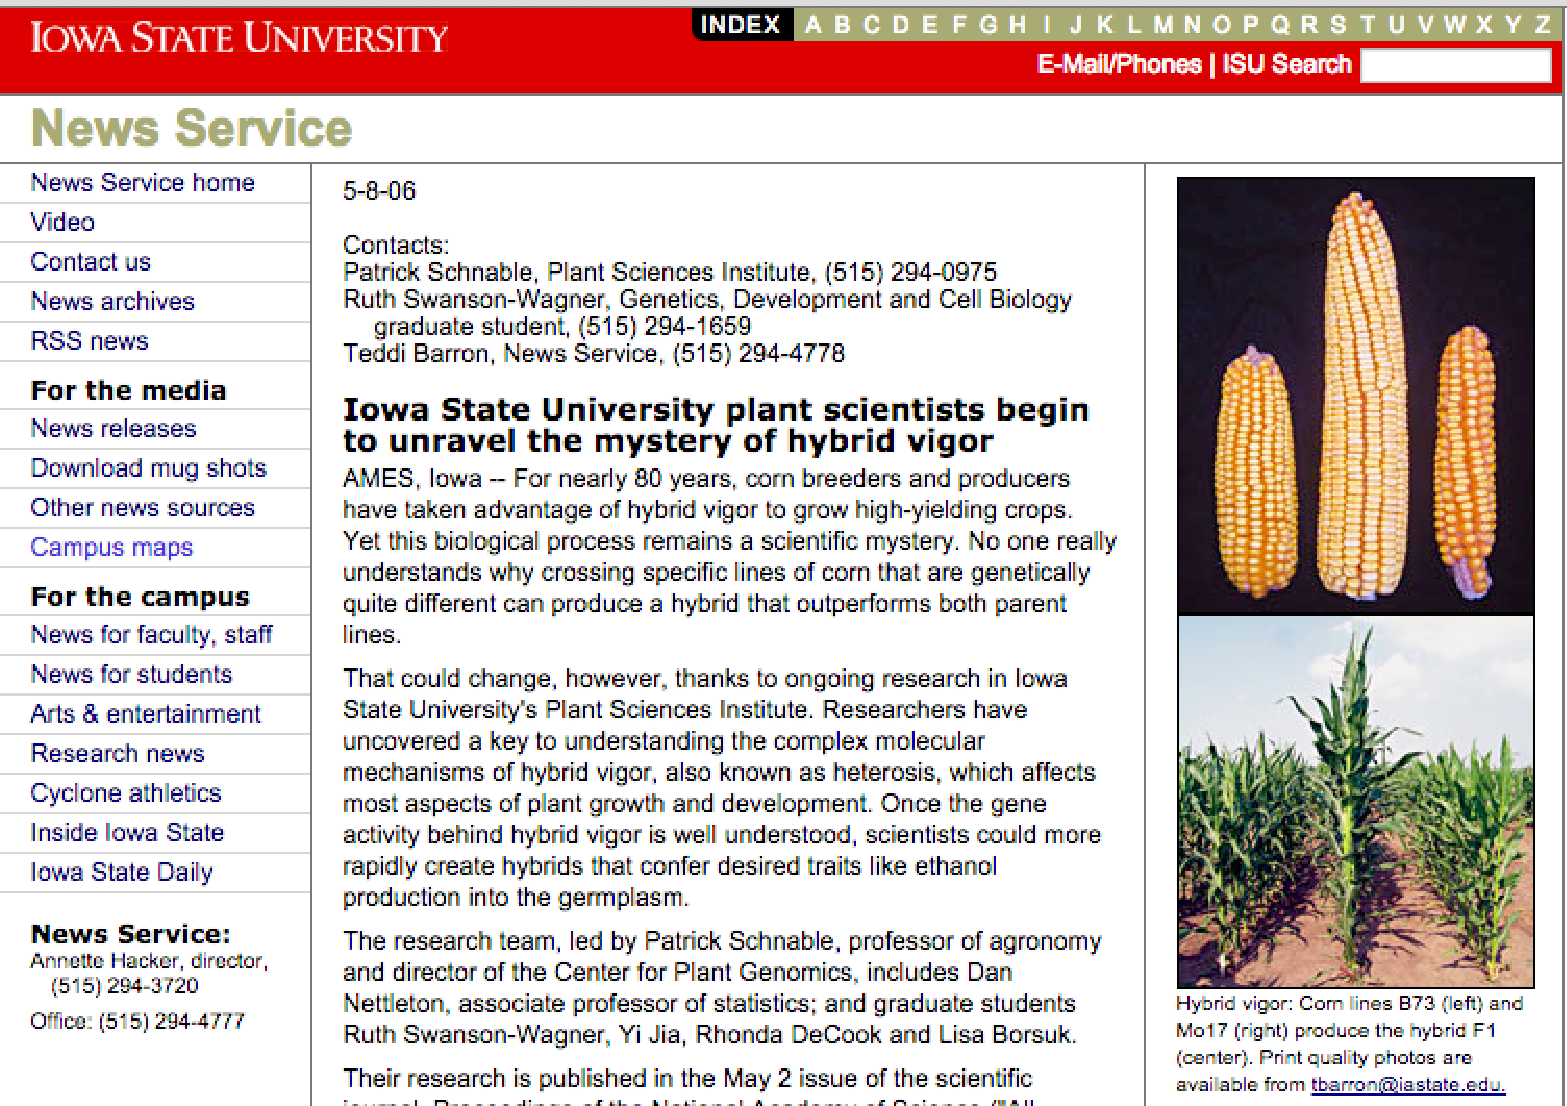
\includegraphics{heterosis_corn}
\end{center}
\end{frame}


\begin{frame}
\frametitle{Phenotypic heterosis in cattle}
\setkeys{Gin}{width=0.8\textwidth}

\vspace{-0.1in}

\begin{center}
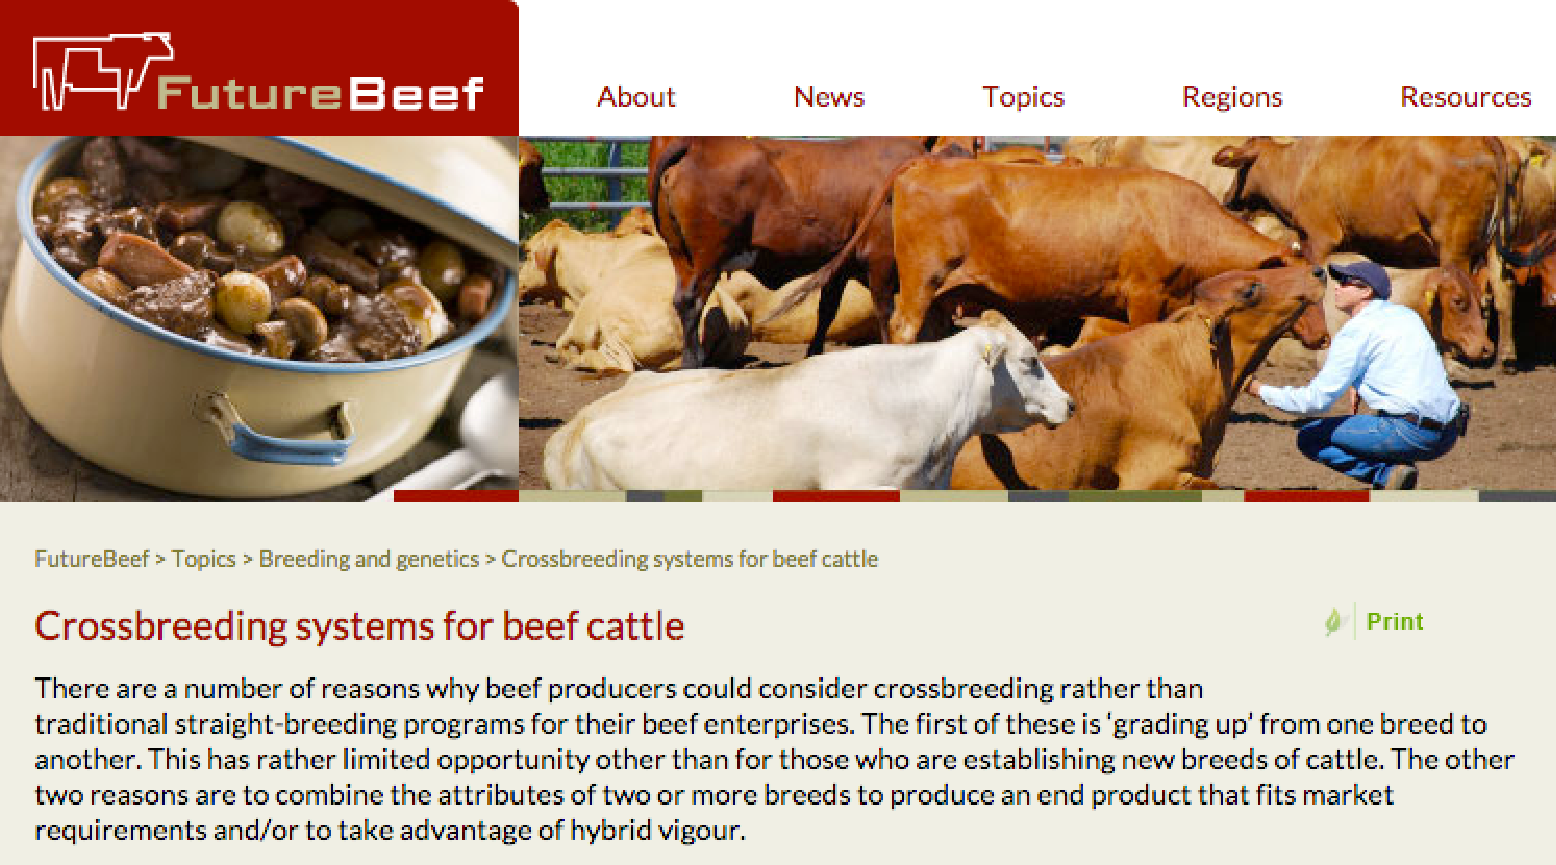
\includegraphics{heterosis_cattle1}

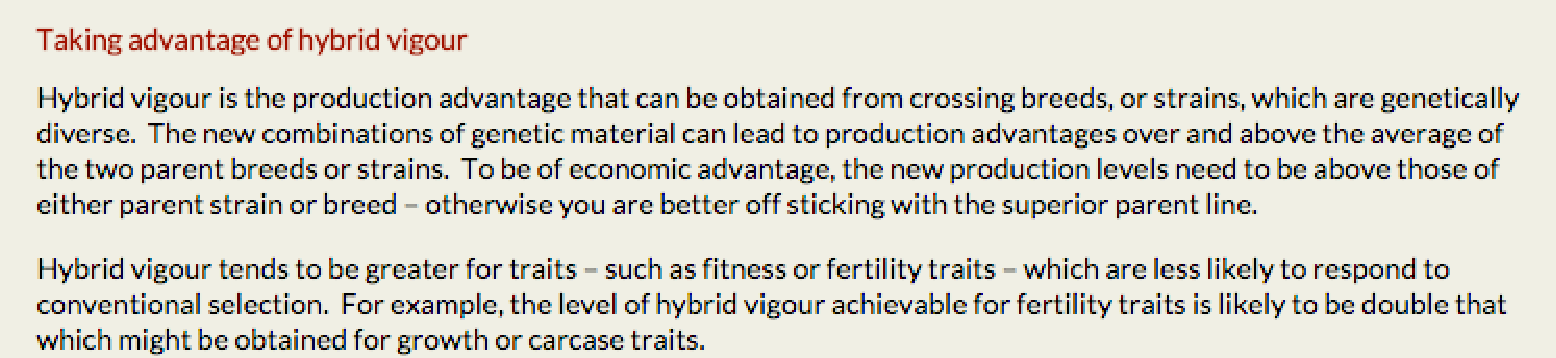
\includegraphics{heterosis_cattle2}
\end{center}
\end{frame}

\subsection{RNAseq experiment}
\begin{frame}
\frametitle{RNAseq experiment}
\setkeys{Gin}{width=0.55\textwidth}

\begin{center}
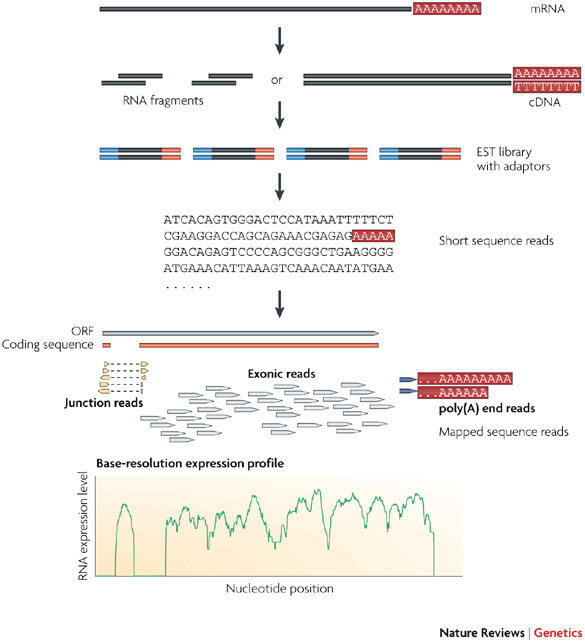
\includegraphics{rnaseq_experiment}
\end{center}

\end{frame}


\begin{frame}
\frametitle{Phenotypic heterosis in RNAseq}
\setkeys{Gin}{width=0.8\textwidth}
\begin{center}
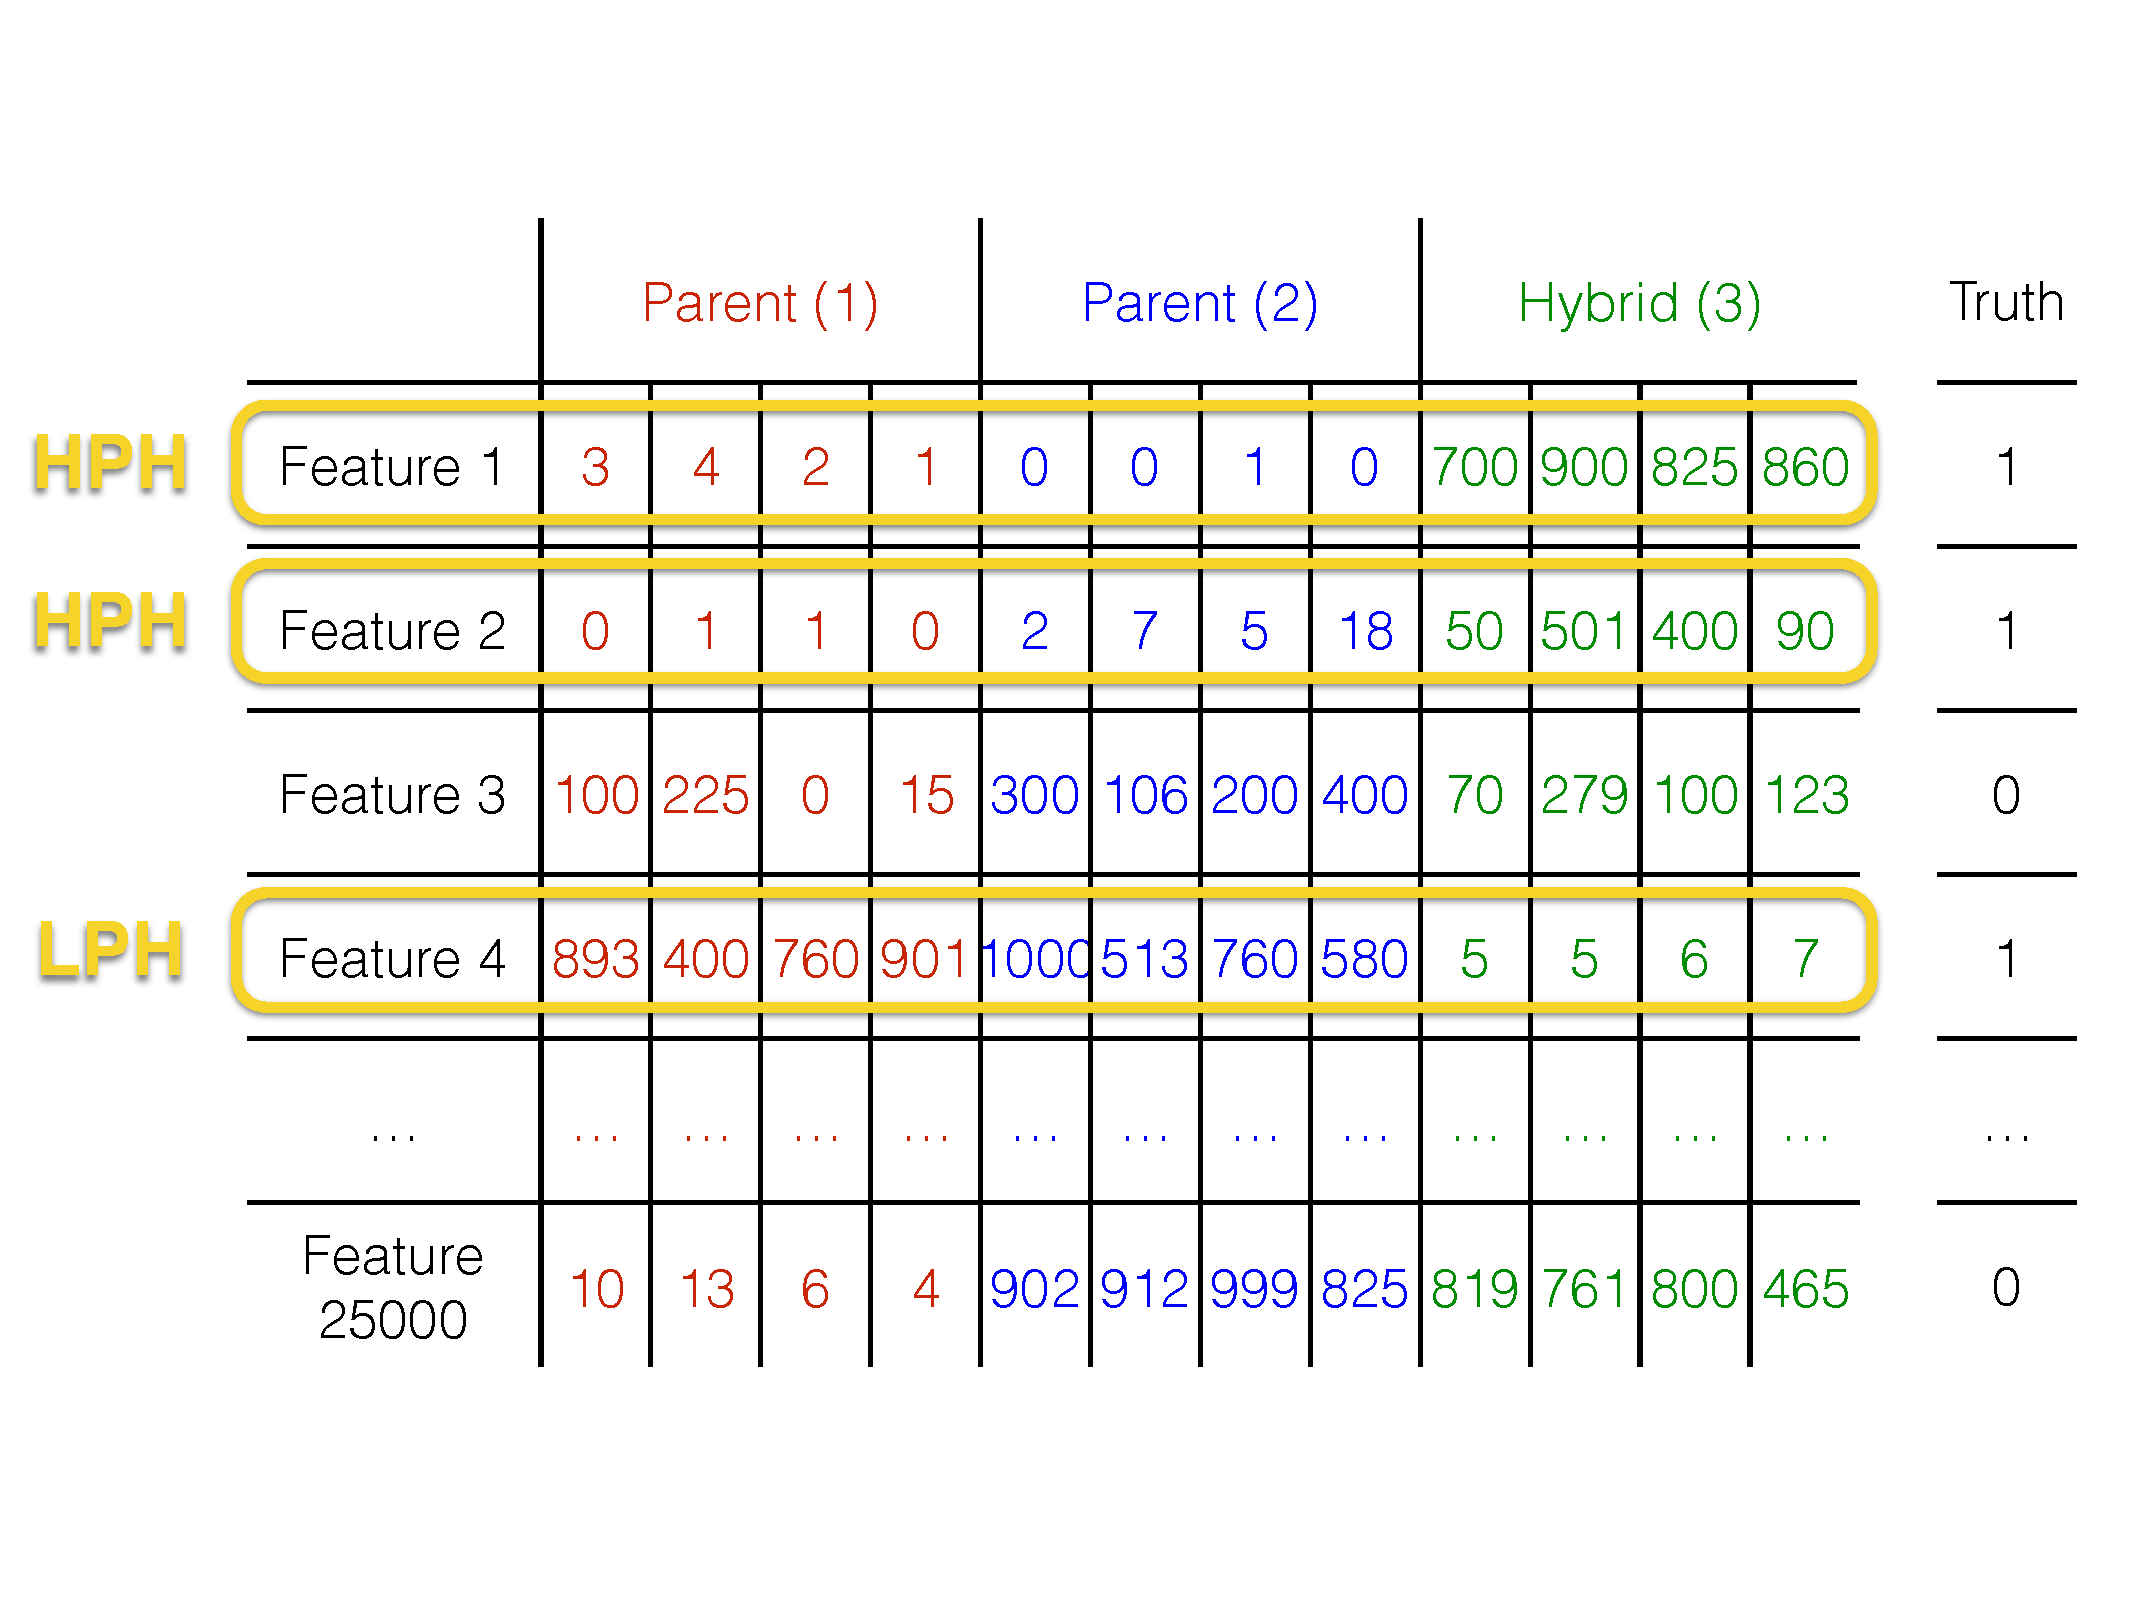
\includegraphics{heterosis_rnaseq}
\end{center}
\end{frame}


\section{Method}
\subsection{Model}

\begin{frame}
\frametitle{RNAseq model}

Let $Y_{gvi}$ be the count for 
\begin{itemize}
\item gene $g=1,\ldots,G$, 
\item variety $v=1,\ldots,V$, and 
\item replicate $i=1,\ldots,n_v$. 
\end{itemize}

\vspace{0.2in} \pause

We assume
\[
Y_{gvi} \stackrel{ind}{\sim} NB\left(e^{\mu_{gv}+c_{vi}},e^{\psi_g}\right) 
\]
\pause
where 
\begin{itemize}
\item $E[Y_{gvi}] = \zeta_{gvi} = e^{\mu_{gv}+c_{vi}}$, \pause 
\item $V[Y_{gvi}] = \zeta_{gvi}+e^{\psi_g}\zeta_{gvi}^2$, \pause and 
\item $c_{vi}$ controls sequencing depth (normalization factors).
\end{itemize}
\end{frame}


\begin{frame}
\frametitle{Reparameterization}
\setkeys{Gin}{width=\textwidth}

Convert the variety specific parameters for parent 1 ($\mu_{g1}$), parent 2 ($\mu_{g2}$), and the hybrid ($\mu_{g3}$) \pause to 

\begin{itemize}[<+->]
\item Parental average: $\phi_g = (\mu_{g1}+\mu_{g2})/2$
\item Half-parental difference: $\alpha_g = (\mu_{g2}-\mu_{g1})/2$
\item Hybrid effect: $\delta_g = \mu_{g3}-\phi_g$
\end{itemize}

\vspace{0.2in} \pause

and thus 
\[ \begin{array}{rl}
\mu_{g1} &= \phi_g + \alpha_g \\
\mu_{g2} &= \phi_g - \alpha_g \\
\mu_{g3} &= \phi_g + \delta_g
\end{array}\]

\pause
\begin{center}
\includegraphics{pad}
\end{center}

\end{frame}



\begin{frame}
\frametitle{Gene expression heterosis}
\setkeys{Gin}{width=\textwidth}

\begin{center}
\includegraphics{pad}
\end{center}
\pause
We define \alert{gene expression heterosis}:

\[ \begin{array}{rll}
H_{g,HPH}: & \delta_g > \phantom{-}|\alpha_g|  & \mbox{high parent heterosis} \pause \\
H_{g,LPH}: & \delta_g < -|\alpha_g|  & \mbox{low parent heterosis} \pause \\
H_{g0}: & |\delta_g| \le  |\alpha_g| 
\end{array} \]

\pause

We are interested in identifying genes with high posterior probabilities for LPH and HPH, i.e. 
\begin{itemize}
\item $P(H_{g,HPH}|y) = P(\delta_g > \phantom{-}|\alpha_g|\, |y)$ and 
\item $P(H_{g,LPH}|y) = P(\delta_g < -|\alpha_g|\, |y)$. 
\end{itemize}

\end{frame}


\begin{frame}[fragile]
\frametitle{Hierarchical model}
\setkeys{Gin}{width=\textwidth}
\begin{itemize}
\item Data model:
\[ Y_{gvi} \stackrel{ind}{\sim} NB\left(e^{\mu_{gv}+c_{vi}},e^{\psi_g}\right) \]
\[ \mu_{g1} = \phi_g + \alpha_g, \mu_{g2} = \phi_g-\alpha_g, \mu_{g3} = \phi_g + \delta_g \]

\pause

\item Hierarchical structure:
\begin{columns}
\begin{column}{0.5\linewidth}
\[ \begin{array}{rl}
\phi_g &\stackrel{ind}{\sim} N(\eta_\phi, \sigma_\phi^2) \\
\alpha_g &\stackrel{ind}{\sim} La(\eta_\alpha, \sigma_\alpha) \\
\delta_g &\stackrel{ind}{\sim} La(\eta_\delta, \sigma_\delta) \\
\psi_g &\stackrel{ind}{\sim} N(\eta_\psi, \sigma_\psi^2) 
\end{array} \]
\end{column} \pause
\begin{column}{0.5\linewidth}
\begin{knitrout}\tiny
\definecolor{shadecolor}{rgb}{0.969, 0.969, 0.969}\color{fgcolor}

{\centering \includegraphics[width=.8\linewidth]{figure/unnamed-chunk-1-1} 

}



\end{knitrout}
\end{column}
\end{columns}
\end{itemize}
\end{frame}


% \begin{frame}[fragile]
% \frametitle{Normal vs Laplace}
% <<>>=
% source("../../sandbox/Laplace.R")
% x = seq(-4,4,by=0.1)
% d = data.frame(rbind(data.frame(density="normal", x=x, y=dnorm(x)),
%                      data.frame(density="Laplace", x=x, y=dlaplace(x,0,sqrt(2)))))
% ggplot(d, aes(x=x,y=y,color=density)) + 
%   geom_line() + 
%   labs(y="f(x)")
% @
% \end{frame}

\subsection{Empirical Bayes}
\begin{frame}
\frametitle{Empirical Bayes}

\begin{enumerate}
\item Estimate hyperparameter, $\pi=(\eta,\sigma,c)$: 

  \begin{enumerate}
  \item Use {\tt edgeR} to obtain $\hat{c}$ and $\hat{\theta}_g = (\hat{\phi}_g,\hat{\alpha}_g,\hat{\delta}_g,\hat{\psi}_g)$. \pause
  \item Use moment matching, to obtain $\hat{\eta}$ and $\hat{\sigma}$.
  \end{enumerate}

\pause
\item Empirical Bayes posterior

\[ p(\theta|y, \hat{\pi}) = \prod_{g=1}^G p(\theta_g|y_g,\hat{\pi}) \]
where $y_g$ is all observations from gene $g$ \pause and 
{\footnotesize
\[ p(\theta_g|y_g,\hat{\pi}) \propto \left[ \prod_{v=1}^V \prod_{i=1}^{n_v} NB\left(y_{gvi};e^{\mu_{gv}+\hat{c}_{vi}}, e^{\psi_g}\right) \right] p\left(\theta_g;\hat{\eta},\hat{\sigma}\right) \]
}
\end{enumerate}
\end{frame}





\subsection{Stan}
\begin{frame}
\frametitle{Stan}
\setkeys{Gin}{width=1\textwidth}

\begin{center}
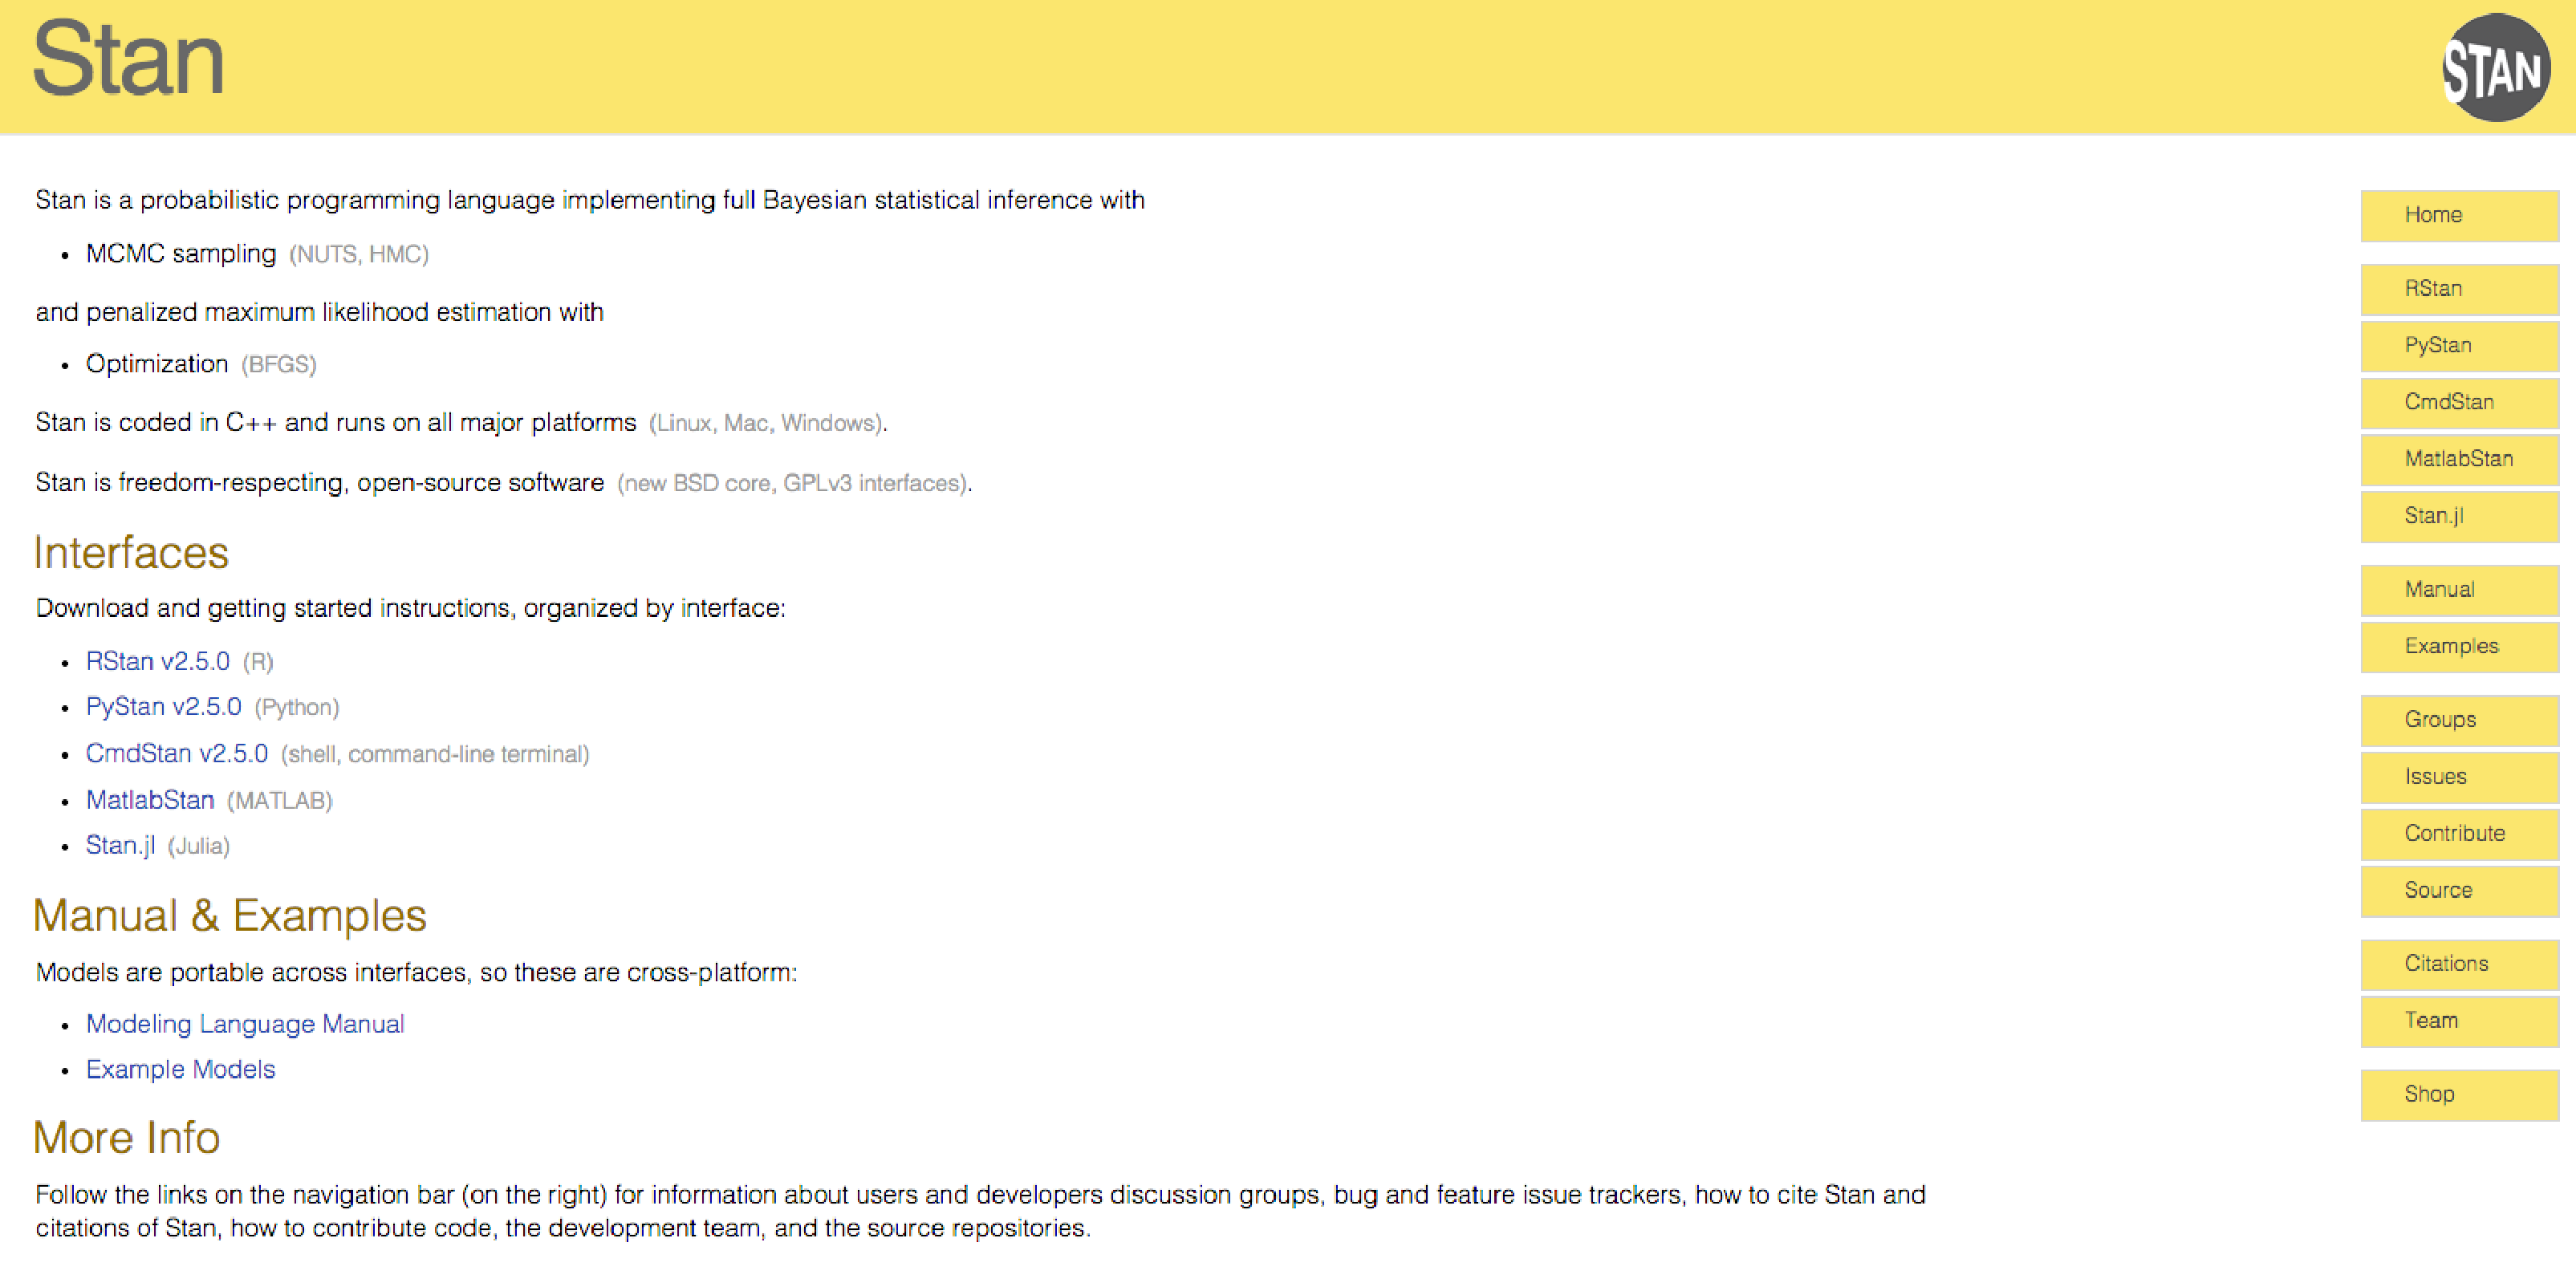
\includegraphics{stan}
\end{center}

For more information, go to \url{http://mc-stan.org/}.

\end{frame}





\begin{frame}[containsverbatim]
\frametitle{}

{\tiny
\begin{verbatim}
data {
  int<lower=1> S;
  int<lower=0> count[S]; 
  int<lower=1,upper=3> variety[S];
  real   eta_phi; real   eta_alpha; real   eta_delta; real   eta_psi; 
  real sigma_phi; real sigma_alpha; real sigma_delta; real sigma_psi;
  vector[S] c;                     // sample sequencing depth
}
transformed data {
  matrix[S,3] X;
  for (s in 1:S) {
    if (variety[s] == 1) { X[s,1] <-  1; X[s,2] <- -1; X[s,3] <-  0; }
    if (variety[s] == 2) { X[s,1] <-  1; X[s,2] <-  1; X[s,3] <-  0; }
    if (variety[s] == 3) { X[s,1] <-  1; X[s,2] <-  0; X[s,3] <-  1; }
  }
}
parameters {
  real phi; real alpha; real delta; real psi;          
}
transformed parameters {
  vector[3] pad;

  pad[1] <- phi;
  pad[2] <- alpha;
  pad[3] <- delta;
}
model {
  phi   ~ normal(            eta_phi,   sigma_phi);
  alpha ~ double_exponential(eta_alpha, sigma_alpha); // Laplace
  delta ~ double_exponential(eta_delta, sigma_delta); // Laplace
  psi   ~ normal(            eta_psi,   sigma_psi);

  count ~ neg_binomial_2_log(X*pad+c, 1/exp(psi));
}
\end{verbatim}
}

\end{frame}


\begin{frame}[fragile]
\frametitle{RStan}

\begin{knitrout}\tiny
\definecolor{shadecolor}{rgb}{0.969, 0.969, 0.969}\color{fgcolor}\begin{kframe}
\begin{alltt}
\hlcom{# set up data}
\hlcom{# ...}
\hlcom{# ...}

\hlcom{# get hyperparameter estimates}
\hlstd{hyperparameter} \hlkwb{=} \hlkwd{get_indep_est}\hlstd{(counts.t,group,geneid.t)}

\hlcom{# change data to long format}
\hlstd{data_stan} \hlkwb{=} \hlkwd{w.to.l}\hlstd{(counts.t,group)}

\hlcom{# compile Stan model (this can take some time, but only needs to be done once)}
\hlstd{sg_model} \hlkwb{=} \hlkwd{stan_model}\hlstd{(}\hlstr{"sg_model.txt"}\hlstd{)}

\hlcom{# use initial values to obtain hyperparameter estimates}
\hlcom{# ...}
\hlcom{# ...}

\hlcom{# loop over all genes}
\hlkwd{library}\hlstd{(doMC)}
\hlkwd{registerDoMC}\hlstd{()}

\hlstd{posterior} \hlkwb{=} \hlkwd{dlply}\hlstd{(stan_data,} \hlkwd{.}\hlstd{(gene),} \hlkwa{function}\hlstd{(}\hlkwc{x}\hlstd{) \{}
  \hlstd{dat} \hlkwb{=} \hlkwd{list}\hlstd{(x, hyperparameter)}
  \hlkwd{sampling}\hlstd{(sg_model, dat,} \hlkwc{chains}\hlstd{=}\hlnum{4}\hlstd{,} \hlkwc{iter}\hlstd{=}\hlnum{2000}\hlstd{)}
\hlstd{\},} \hlkwc{.parallel}\hlstd{=}\hlnum{TRUE}\hlstd{)}
\end{alltt}
\end{kframe}
\end{knitrout}

\end{frame}


\section{Results}
\subsection{Simulation study}
\begin{frame}
\frametitle{Simulation study}

Simulation study:
\begin{enumerate}[<+->]
\item Used {\tt edgeR} to estimate $\theta_g$ and $c$ (about 30\% have heterosis)
\item Simulated data from a negative binomial model using the estimated $\theta_g$ and $c$
\item Used each method below to rank genes according to plausibility of heterosis
\item Compared methods based on receiving operating characteristic (ROC) curves
\end{enumerate}

\vspace{0.2in} \pause

Compared our method to 
\begin{itemize}
\item {\tt edgeR}, 
\item {\tt baySeq}, 
\item Ji et. al. log(count+1)
\item {\tt ShrinkBayes} - INLA
\end{itemize}

\end{frame}



\subsection{ROC curves}
\begin{frame}
\frametitle{Example ROC curve}
\setkeys{Gin}{width=\textwidth}
\begin{center}
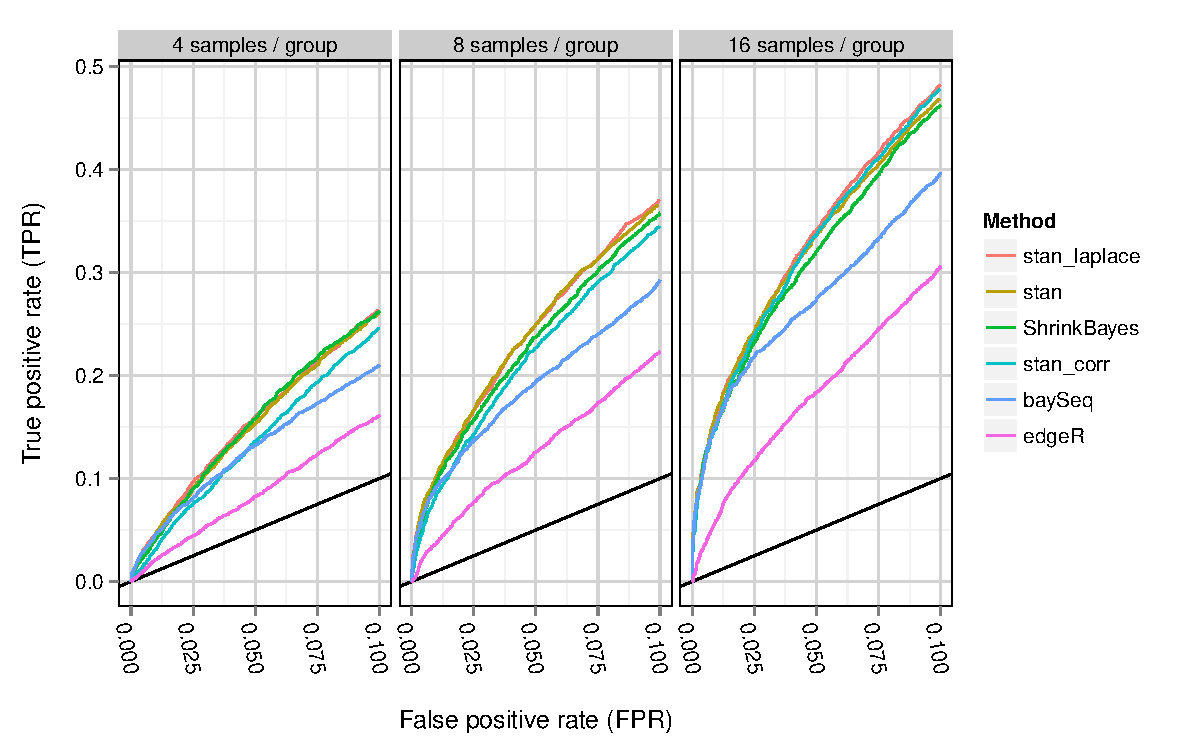
\includegraphics{exampleROC0_1}
\end{center}
\end{frame}


\begin{frame}
\frametitle{Area under ROC curve}
\setkeys{Gin}{width=\textwidth}
\begin{center}
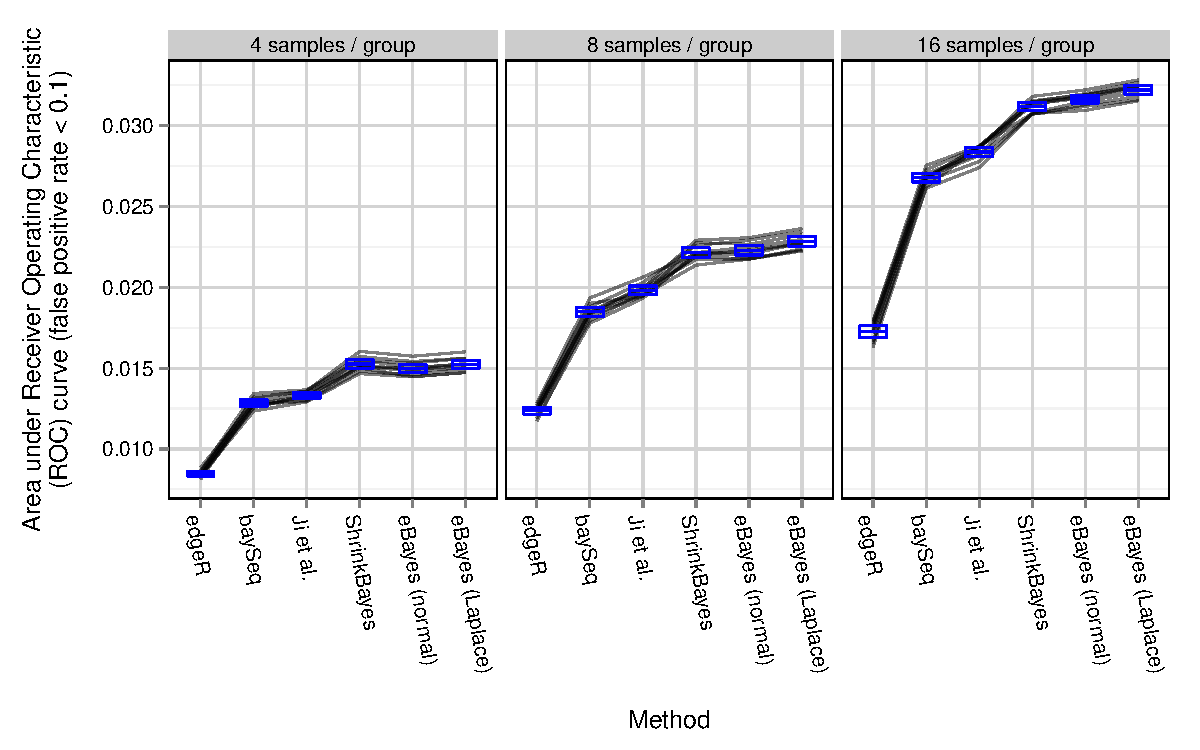
\includegraphics{auc-facet-TRUE}
\end{center}
\end{frame}


\begin{frame}
\frametitle{Evaluation of empirical Bayes estimates}

In this simulation study, we have no true hyperparameters. \pause But we can evaluate how good our hyperparameters are in estimating means and standard deviations of the gene-specific parameters, \pause e.g. 
\[ 
\eta_\alpha^{\mbox{truth}} \equiv \frac{1}{G} \sum_{g=1}^G \alpha_g^{\mbox{edgeR}} \pause \qquad 
\sigma_\alpha^{2\mbox{truth}} \equiv \frac{1}{G} \sum_{g=1}^G \left( \alpha_g^{\mbox{edgeR}} - \eta_\alpha^{\mbox{truth}}\right)^{2}
\]

\pause

{\tiny
% latex table generated in R 3.2.1 by xtable 1.7-4 package
% Fri Sep  4 15:08:19 2015
\begin{table}[ht]
\centering
\caption{RMSE for hyperparameter estimates across the 10 simulations.} 
\label{t:hyperparameter}
\begin{tabular}{lrrrr}
  \hline
& & \multicolumn{3}{c}{Reps per variety} \\
Parameter & Truth & 4 & 8 & 16 \\ 
  \hline
$\eta_\phi$ & 3.440 & 0.005 & 0.006 & 0.009 \\ 
  $\eta_\alpha$ & -0.051 & 0.003 & 0.004 & 0.002 \\ 
  $\eta_\delta$ & 0.078 & 0.022 & 0.023 & 0.023 \\ 
  $\eta_\psi$ & -2.345 & 0.114 & 0.073 & 0.041 \\ 
   \hline
$\sigma_\phi$ & 2.736 & 0.001 & 0.006 & 0.006 \\ 
  $\sigma_\alpha$ & 0.363 & 0.018 & 0.004 & 0.002 \\ 
  $\sigma_\delta$ & 0.328 & 0.086 & 0.043 & 0.022 \\ 
  $\sigma_\psi$ & 0.599 & 0.192 & 0.099 & 0.049 \\ 
   \hline
\end{tabular}
\end{table}

}
\end{frame}






\subsection{Real data analysis}
\begin{frame}
\frametitle{Real data analysis}

We used our method to analyze a maize data set of RNA-seq gene expression in parental lines B73 and Mo17 and the hybrid genotype (B73$\times$Mo17) with a total of 39,656 genes.

\vspace{0.2in} \pause

Analysis proceeds by 
\begin{itemize}
\item Estimate hyperparameters $\hat{\pi}$
\item In parallel, gene-specific analyses for certain genes\pause, e.g. 
\[ 
\left| \delta_g^{edgeR}\right| > \left| \alpha_g^{edgeR}\right| 
\]
which was 30\% of the original genes.
\end{itemize}
\end{frame}





\begin{frame}
\frametitle{Shrinkage}
\begin{center}
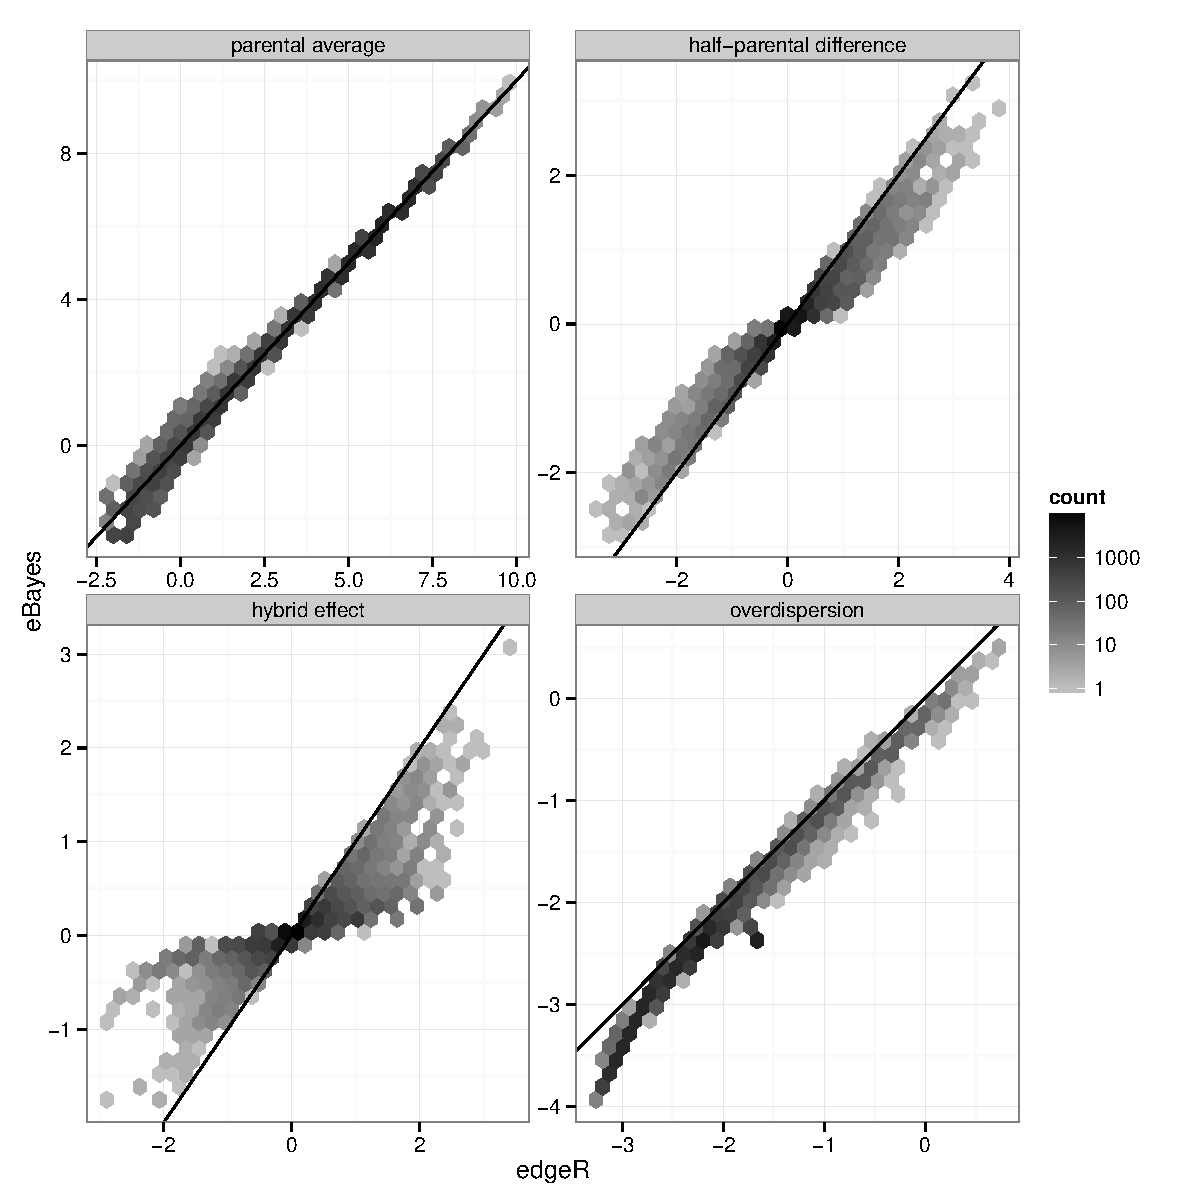
\includegraphics{gene_specific_estimates}
\end{center}
\end{frame}

% \begin{frame}
% \frametitle{Estimates}
% \begin{center}
% 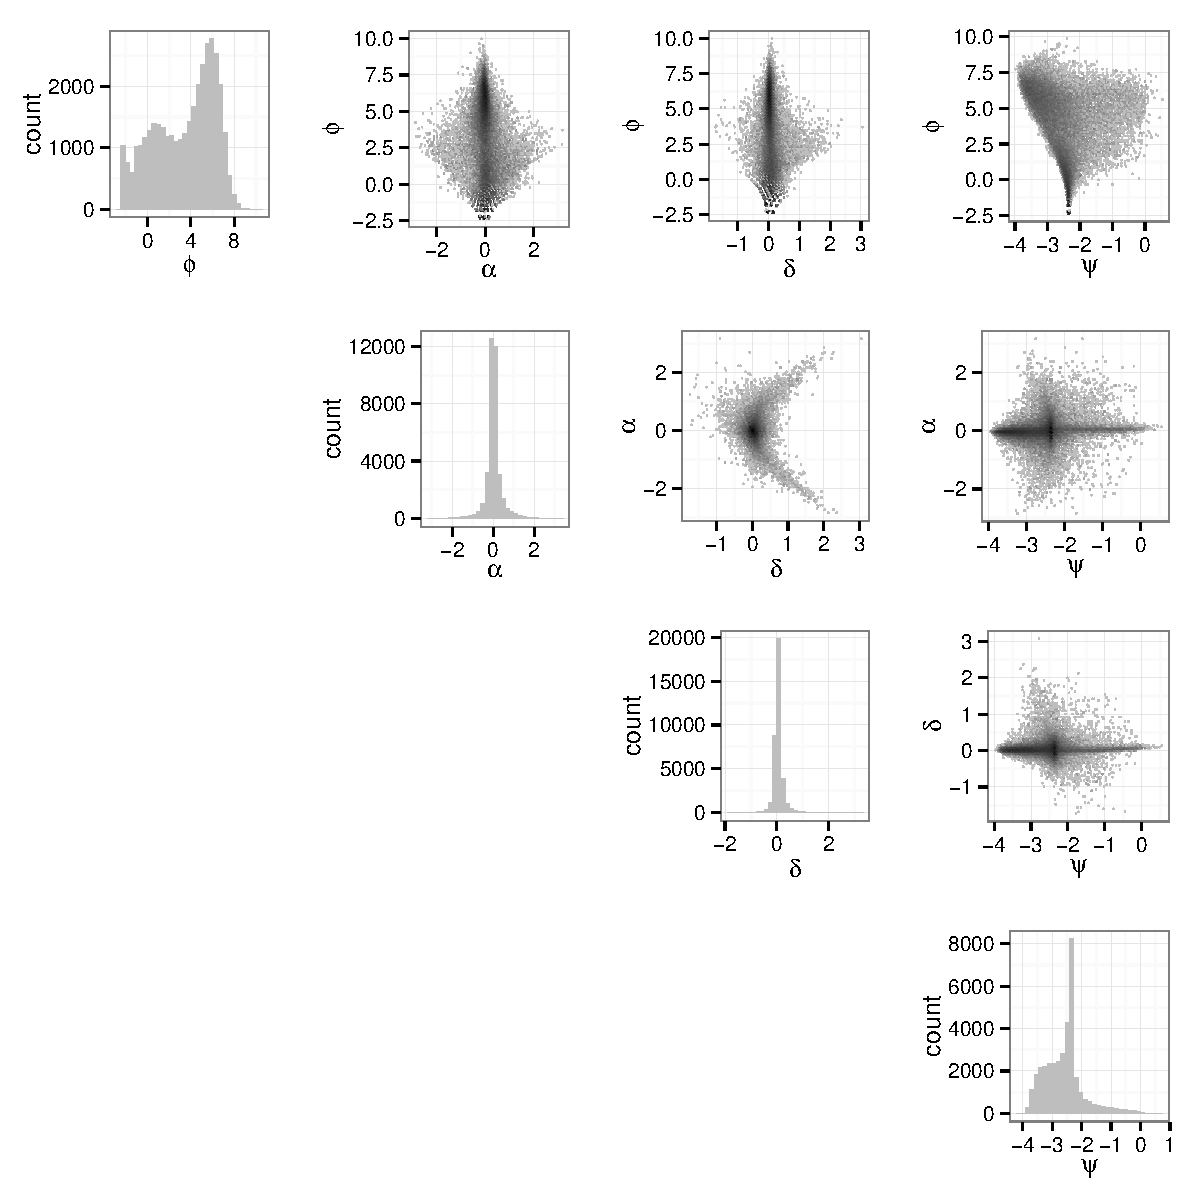
\includegraphics{estimates}
% \end{center}
% \end{frame}




\begin{frame}
\frametitle{Volcano plot for real data}
\setkeys{Gin}{width=0.6\textwidth}
\begin{center}
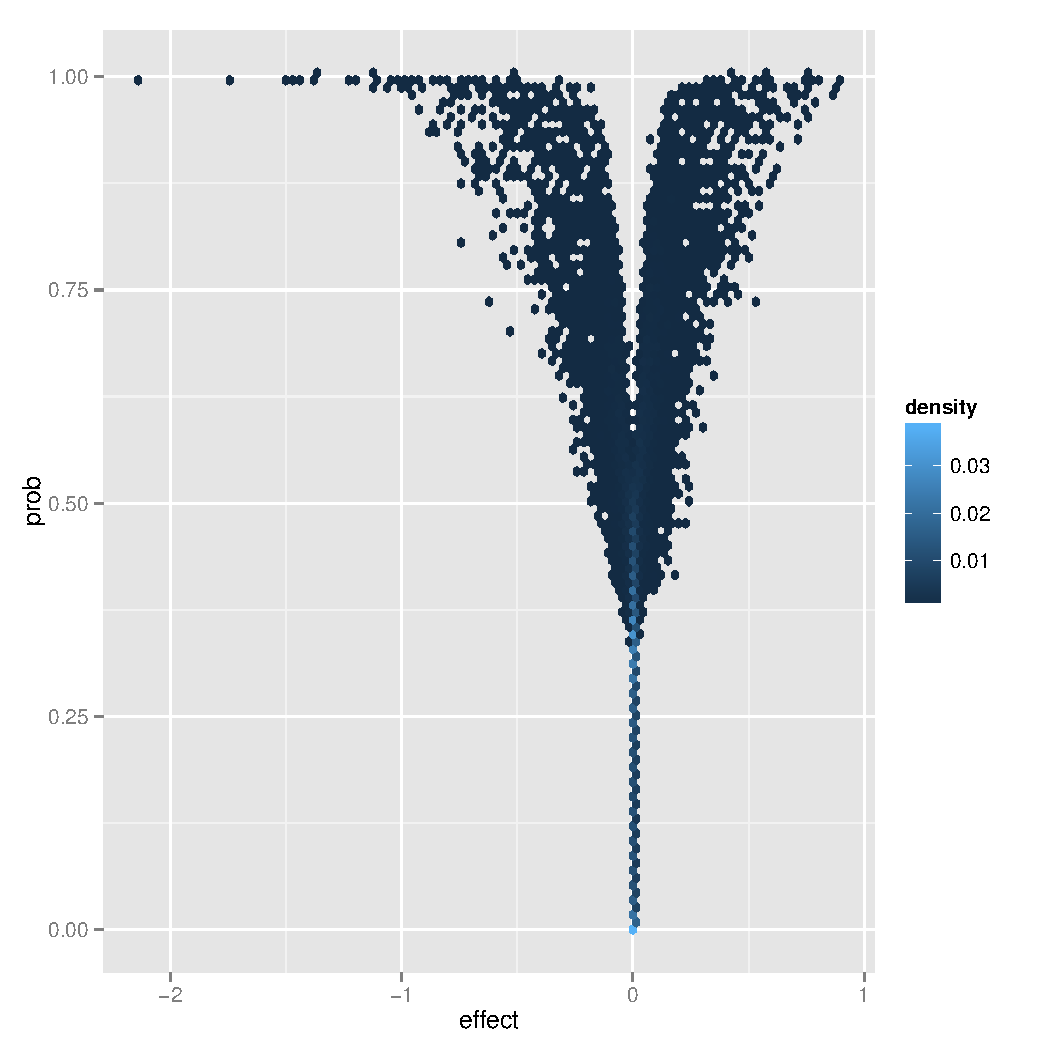
\includegraphics{volcano}
\end{center}
\end{frame}


\begin{frame}
\frametitle{eBayes heterosis for RNAseq}

Jarad Niemi , Eric Mittman, Will Landau, Dan Nettleton. (2015) Empirical Bayes Analysis of RNA-seq Data for Detection of Gene Expression Heterosis. \emph{Journal of Agricultural, Biological, and Environmental Statistics}. December 2015, Volume 20, Issue 4, pp 614-628

\end{frame}



\section{Fully Bayesian analysis}
\begin{frame}
\frametitle{Fully Bayesian analysis}

An MCMC implementation:
\begin{enumerate}
\item Independently, sample $\phi_g \sim (\phi_g|\ldots)$ for $g=1,\ldots,G$.
\item Independently, sample $\alpha_g \sim (\alpha_g|\ldots)$ for $g=1,\ldots,G$.
\item Independently, sample $\delta_g \sim (\delta_g|\ldots)$ for $g=1,\ldots,G$.
\item Independently, sample $\psi_g \sim (\psi_g|\ldots)$ for $g=1,\ldots,G$.

\vspace{0.1in} \pause

\item Sample hyperparameters:
\begin{itemize}
\item $\eta_\phi,\sigma_\phi^2$ depend on summary \emph{statistics} of $(\phi_1,\ldots,\phi_G)$.
\item $\eta_\alpha,\sigma_\alpha^2$ depend on summary \emph{statistics} of $(\alpha_1,\ldots,\alpha_G)$.
\item $\eta_\delta,\sigma_\delta^2\,$ depend on summary \emph{statistics} of $(\delta_1,\ldots,\delta_G)$.
\item $\eta_\psi,\sigma_\psi^2$ depend on summary \emph{statistics} of $(\psi_1,\ldots,\psi_G)$.
\end{itemize}
\end{enumerate}

\vspace{0.1in} \pause

The problem is that $G$ is large, i.e. ~40k.

\end{frame}


\begin{frame}
\frametitle{Parallel reduction}

A serial sum of $G$ numbers, e.g. $\sum_{g=1}^G \delta_g$, has a computational complexity of $O(G)$. \pause
A parallel reduction has computational complexity of $O\left(\frac{G}{S} \log_2(G) \right)$ where $S$ is ``speedup'', i.e. the number of parallel processes we have. 

\vspace{0.2in} \pause

\begin{center}
\includegraphics{parallel_reduction}
\end{center}

\end{frame}



\begin{frame}
\frametitle{Computational tractibility via parallelism}

Amdahl's Law:
\[
\mbox{speedup} = \frac{1}{1-P+\frac{P}{S}}
\]
\pause
where
\begin{itemize}
\item $P$ is the proportion of the execution time that would benefit from speed up
\item $S$ is the speedup of that proportion
\end{itemize}

\vspace{0.2in} \pause

Parallel hardware
\begin{itemize}[<+->]
\item Multi-CPU/multi-core
\item Cluster
\item Graphical processing units (GPUs)
\begin{itemize}
\item Minimize memory transfer between host (CPU) and device (GPU)
\item Only have uniform and normal samplers
\end{itemize}
\end{itemize}
\end{frame}


\begin{frame}
\frametitle{Minimizing data transfer}

Since there are $4G+8\approx 160,000$ parameters, it is not feasible to return MCMC samples for all parameters. \pause We typically need samples to 
\begin{itemize}
\item Assess convergence
\item Perform inference
\end{itemize}

\vspace{0.2in} \pause

Instead, return relevant summary quantities:
\begin{itemize}
\item Convergence for $\psi$
  \begin{itemize}
  \item $\psi$ sum
  \item $\psi^2$ sum 
  \end{itemize}
\item Inference for $\psi$
  \begin{itemize}
  \item $\psi$ sum
  \item $\psi^2$ sum 
  \end{itemize}
\end{itemize}
\end{frame}



\begin{frame}
\frametitle{Assessing convergence}
Assessing convergence for a quantity of interest $\psi$ using potential scale reduction factor using $M$ chains each with $N$ samples: \pause
\[ 
\hat{R} = 
%\widehat{\mbox{var}}^+(\psi|y) = 
\frac{N-1}{N}W + \frac{1}{N}B
\]
\pause
where
\[ \begin{array}{rl}
B &= \frac{N}{M-1}\sum_{m=1}^M \left(\overline{\psi}_{\cdot m} - \overline{\psi}_{\cdot \cdot}\right)^2 \\
W &= \frac{1}{M}\sum_{m=1}^M s_m^2
\end{array} \]
\pause
and 
\[ \begin{array}{rl}
\overline{\psi}_{\cdot m} & = \frac{1}{N} \sum_{n=1}^N \psi_{nm} \\
\overline{\psi}_{\cdot \cdot} &= \frac{1}{M} \sum_{m=1}^M \overline{\psi}_{\cdot m} \\
s_m^2 &= \frac{1}{N-1} \sum_{n=1}^N \left(\psi_{nm} -\overline{\psi}_{\cdot m} \right)^2 \pause = \frac{1}{N-1} \sum_{n=1}^N \psi_{nm}^2 - \frac{N}{N-1} \overline{\psi}_{\cdot m}^2
\end{array} \]
\end{frame}


\begin{frame}
\frametitle{Inference}

There are two main types of quantities of interest:
\begin{itemize}
\item Parameters, e.g. $\delta_g$ or $\theta_\delta$
\item Functions of parameters, e.g. $\mathrm{I}(\delta_g > |\alpha_g|)$
\end{itemize}
\pause
For both situations, we keep a running sum, e.g. 
\begin{itemize}
\item $\sum_{n=1}^N \delta_{g,n}$ 
\item $\sum_{n=1}^N \mathrm{I}(\delta_{g,n} > |\alpha_{g,n}|)$
\end{itemize}
\pause
Two caveats:
\begin{itemize}
\item Must pre-specify all quantities of interest.
\item Cannot calculate MCMC SE.
\end{itemize}
\end{frame}



\begin{frame}
\frametitle{Slice sampling}

GPUs only have normal and uniform samplers. 
\pause 
The only full conditional that is normal or uniform is $\theta_\cdot$. 
\pause 
For all other parameters, we use slice sampling.  
\pause
The identity
\[
p(\psi|\ldots) = \int_0^{p(\psi|\ldots)} du
\]
\pause
implies the joint distribution
\[ 
p(\psi,u|\ldots) \propto \mathrm{I}(0<u<p(\psi|\ldots))
\]
\pause
which has the following full conditional distributions
\begin{itemize}
\item $U|\ldots \sim Unif(0,p(\psi|\ldots))$ \pause
\item $\psi|\ldots \sim Unif\{\psi:u<p(\psi|\ldots)\}$
\end{itemize}
\pause
The difficulty is in finding the set $\{\psi:u<p(\psi|\ldots)\}$.
\end{frame}



\begin{frame}
\frametitle{Stepping-out slice sampler}

To sample from $p(\psi|u,\ldots)$, let 
\begin{itemize}
\item $u^{(n)}$ be the current draw for the auxiliary variable $u$ \pause
\item $\psi^{(n-1)}$ be the current draw for $\psi$, \pause and we know $u^{(n)}<p(\psi^{(n-1)}|\ldots)$ \pause
\item $w$ be a tuning parameter that you choose
\end{itemize}
\pause
Perform the following
\begin{enumerate}
\item Randomly place an interval $(\psi_L(u^{(n)}),\psi_U(u^{(n)}))$ of length $w$ around the current value $\psi^{(i-1)}$. \pause
\item Step the endpoints of this interval out in increments of $w$ until $u^{(n)}>p(\psi_L(u^{(n)})|\ldots)$ and $u^{(n)}>p(\psi_B(u^{(n)})|\ldots)$. \pause
\item Sample $\psi^* \sim Unif(\psi_L(u^{(n)}),\psi_L(u^{(n)}))$. \pause
\item If $u^{(n)}<p(\psi^*|\ldots)$, then set $\psi^{(n)} = \psi^*$, \pause otherwise
  \begin{enumerate}
  \item set $\psi_L(u^{(n)}) = \psi^*$ if $\psi^* <  \psi^{(n-1)}$ or
  \item set $\psi_U(u^{(n)}) = \psi^*$ if $\psi^* > \psi^{(n-1)}$ \pause and
  \item return to Step 3.
  \end{enumerate}
\end{enumerate}
\end{frame}




\begin{frame}
\frametitle{}
\begin{knitrout}\tiny
\definecolor{shadecolor}{rgb}{0.969, 0.969, 0.969}\color{fgcolor}

{\centering \includegraphics[width=.8\linewidth]{figure/stepping_out_examples-1} 

}



\end{knitrout}
\end{frame}



\begin{frame}
\frametitle{Fully Bayesian analysis}

With $G=40,000$ genes with $V=3$ varieties and $n_v=4$ replicates per variety, \pause 
after 24 hours of running the GPU version of this fully Bayesian analysis, \pause 
we have apparent convergence for all parameters of interest except a handful of gene-specific parameters ($\hat{R}\approx 1.15$). 

\vspace{0.2in} \pause 

Comments:
\begin{itemize}[<+->]
\item With so many parameters, there is reasonably high probability that some will show lack of convergence.
\item If we remove these genes, all remaining parameters appear to converge. 
\item These genes will have minimal impact on inference for hyperparameters and all other genes. 
\end{itemize}


\end{frame}


\begin{frame}
\frametitle{Bottom line:}

\begin{itemize}[<+->]
\item A fully Bayesian analysis will incorporate more of our uncertainty.
\item It may justify our (or another) empirical Bayes approach. 
\end{itemize}

\vspace{0.5in} \pause

\begin{center}
{\Huge
Thank you!
}
\end{center}

\end{frame}


\end{document}
